\section{ConnectionWrapper Class Reference}
\label{classConnectionWrapper}\index{ConnectionWrapper@{ConnectionWrapper}}
{\tt \#include $<$connectionwrapper.h$>$}

Inheritance diagram for ConnectionWrapper:\nopagebreak
\begin{figure}[H]
\begin{center}
\leavevmode
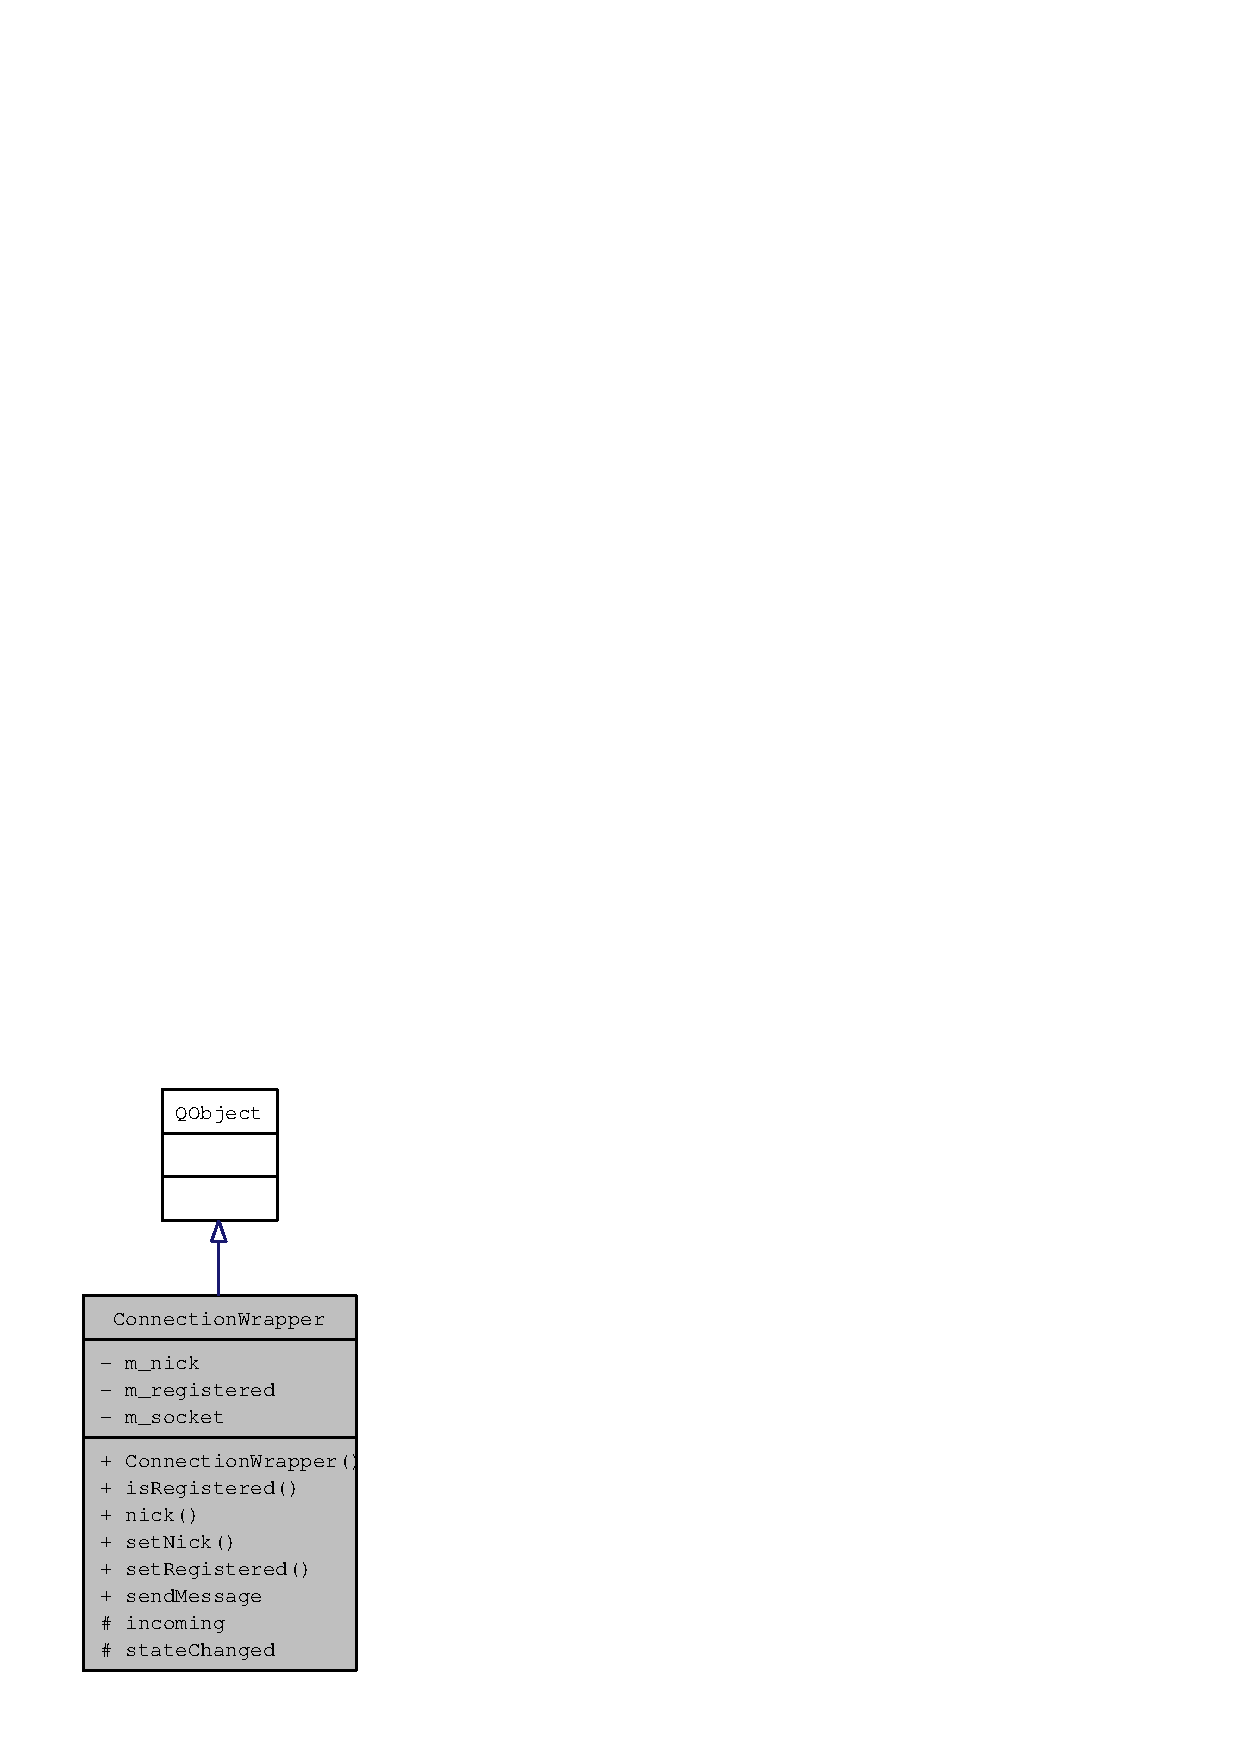
\includegraphics[width=87pt]{classConnectionWrapper__inherit__graph}
\end{center}
\end{figure}
Collaboration diagram for ConnectionWrapper:\nopagebreak
\begin{figure}[H]
\begin{center}
\leavevmode
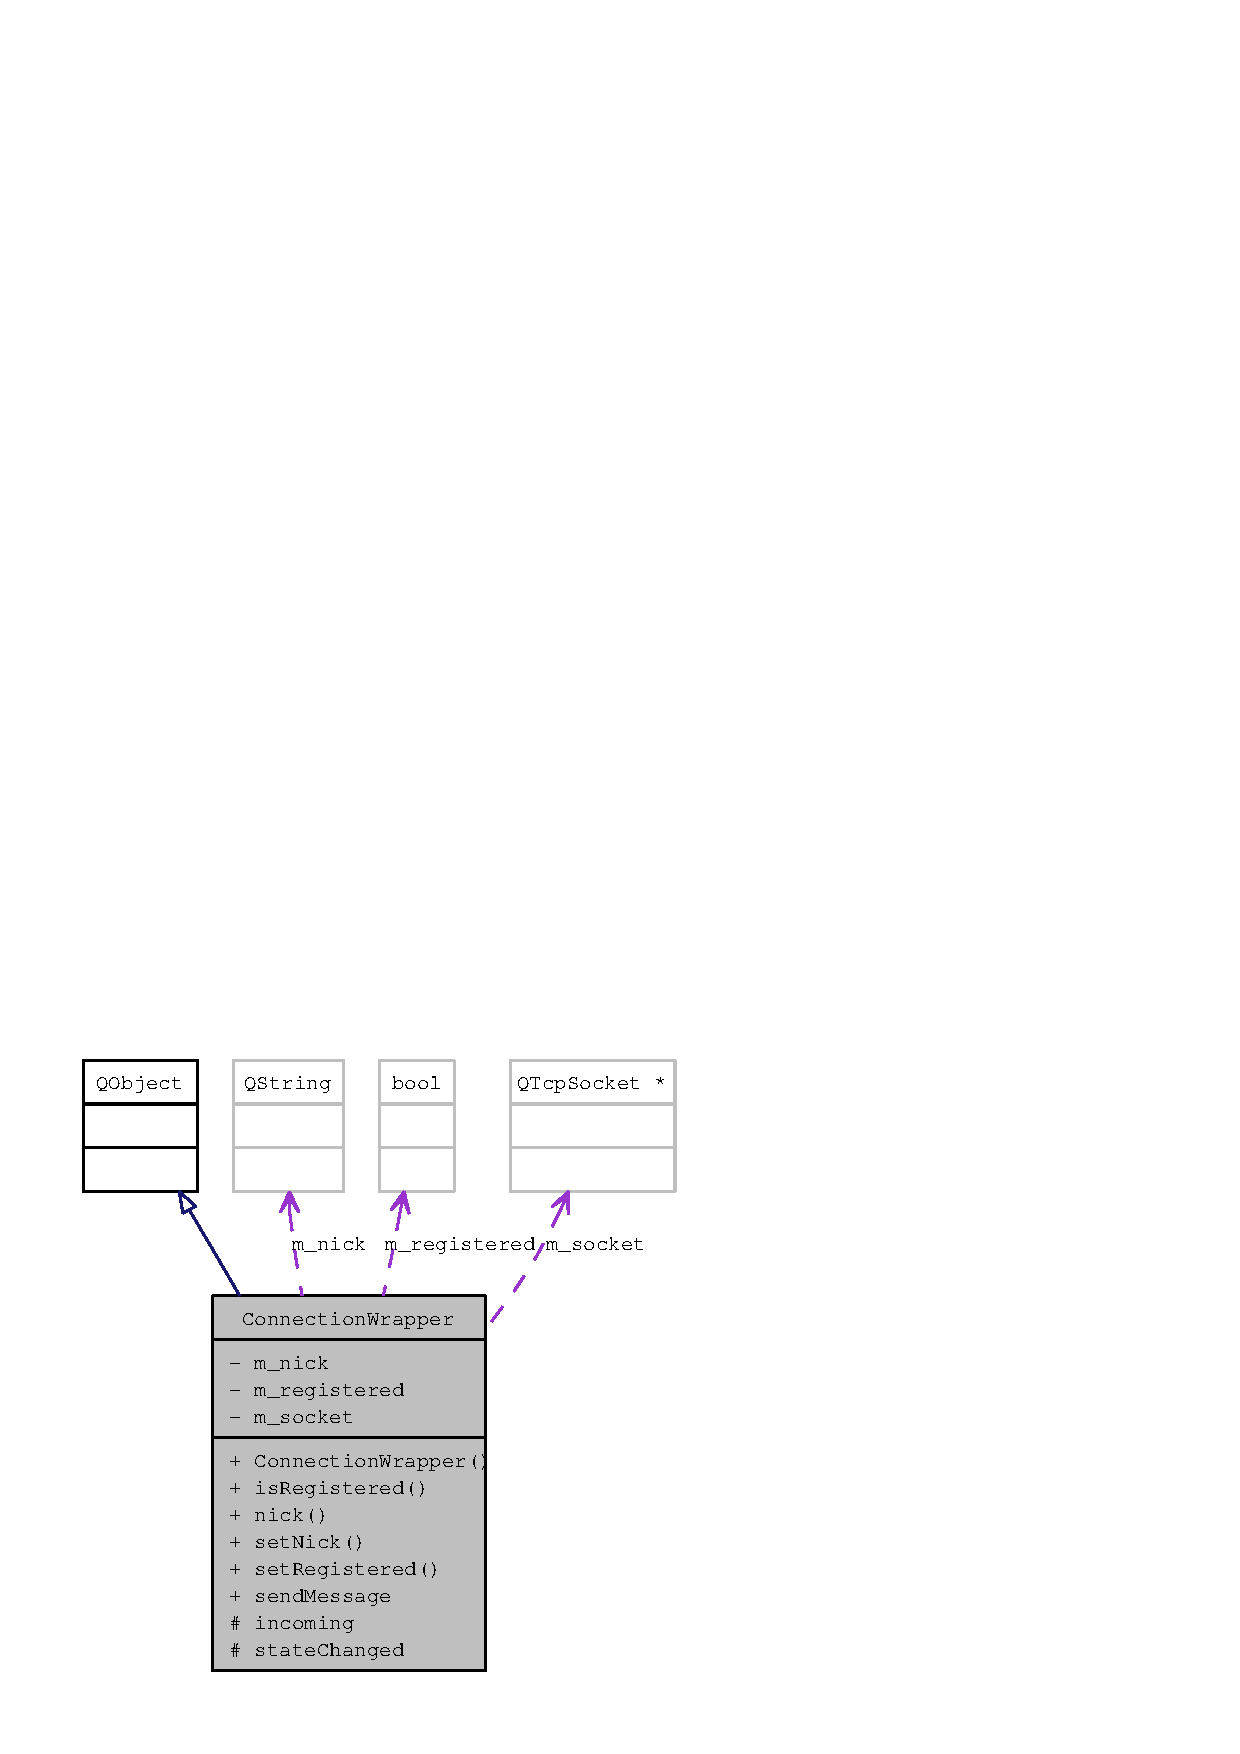
\includegraphics[width=163pt]{classConnectionWrapper__coll__graph}
\end{center}
\end{figure}
\subsection*{Public Slots}
\begin{CompactItemize}
\item 
void {\bf sendMessage} (const QString \&message)
\end{CompactItemize}
\subsection*{Signals}
\begin{CompactItemize}
\item 
void {\bf gotMessage} (const QString \&message)
\end{CompactItemize}
\subsection*{Public Member Functions}
\begin{CompactItemize}
\item 
{\bf ConnectionWrapper} (QTcpSocket $\ast$socket, {\bf QObject} $\ast$parent=0)
\item 
bool {\bf isRegistered} () const 
\item 
QString {\bf nick} () const 
\item 
void {\bf setNick} (QString nick)
\item 
void {\bf setRegistered} (bool registered)
\end{CompactItemize}
\subsection*{Protected Slots}
\begin{CompactItemize}
\item 
void {\bf incoming} ()
\item 
void {\bf stateChanged} (QAbstractSocket::SocketState)
\end{CompactItemize}
\subsection*{Private Attributes}
\begin{CompactItemize}
\item 
QString {\bf m\_\-nick}
\item 
bool {\bf m\_\-registered}
\item 
QTcpSocket $\ast$ {\bf m\_\-socket}
\end{CompactItemize}


\subsection{Detailed Description}


Definition at line 9 of file connectionwrapper.h.

\subsection{Constructor \& Destructor Documentation}
\index{ConnectionWrapper@{ConnectionWrapper}!ConnectionWrapper@{ConnectionWrapper}}
\index{ConnectionWrapper@{ConnectionWrapper}!ConnectionWrapper@{ConnectionWrapper}}
\subsubsection{\setlength{\rightskip}{0pt plus 5cm}ConnectionWrapper::ConnectionWrapper (QTcpSocket $\ast$ {\em socket}, {\bf QObject} $\ast$ {\em parent} = {\tt 0})}\label{classConnectionWrapper_9fb601f65a6f81e37f55a1cb61dcedd0}




Definition at line 5 of file connectionwrapper.cpp.

References incoming(), m\_\-socket, and stateChanged().

\begin{Code}\begin{verbatim}6                   :QObject(parent), m_socket(socket), m_registered(false)
7 {
8     connect(m_socket, SIGNAL(disconnected()),
9             this, SLOT(deleteLater()));
10     connect(m_socket, SIGNAL(readyRead()),
11             this, SLOT(incoming()));
12     connect(socket, SIGNAL(stateChanged(QAbstractSocket::SocketState)),
13             this, SLOT(stateChanged(QAbstractSocket::SocketState)));
14 }
\end{verbatim}
\end{Code}




\subsection{Member Function Documentation}
\index{ConnectionWrapper@{ConnectionWrapper}!gotMessage@{gotMessage}}
\index{gotMessage@{gotMessage}!ConnectionWrapper@{ConnectionWrapper}}
\subsubsection{\setlength{\rightskip}{0pt plus 5cm}void ConnectionWrapper::gotMessage (const QString \& {\em message})\hspace{0.3cm}{\tt  [signal]}}\label{classConnectionWrapper_9f4380ec379556532682fa776174daef}




Referenced by incoming().\index{ConnectionWrapper@{ConnectionWrapper}!incoming@{incoming}}
\index{incoming@{incoming}!ConnectionWrapper@{ConnectionWrapper}}
\subsubsection{\setlength{\rightskip}{0pt plus 5cm}void ConnectionWrapper::incoming ()\hspace{0.3cm}{\tt  [protected, slot]}}\label{classConnectionWrapper_2a71069fecee1f382b9ac7947bc29736}




Definition at line 22 of file connectionwrapper.cpp.

References gotMessage(), and m\_\-socket.

Referenced by ConnectionWrapper().

\begin{Code}\begin{verbatim}23 {
24     while (m_socket->canReadLine()) {
25         QByteArray data = m_socket->readLine();
26         QString line = QString::fromUtf8(data.data(), data.size());
27         emit gotMessage(line);
28     }
29 }
\end{verbatim}
\end{Code}


\index{ConnectionWrapper@{ConnectionWrapper}!isRegistered@{isRegistered}}
\index{isRegistered@{isRegistered}!ConnectionWrapper@{ConnectionWrapper}}
\subsubsection{\setlength{\rightskip}{0pt plus 5cm}bool ConnectionWrapper::isRegistered () const\hspace{0.3cm}{\tt  [inline]}}\label{classConnectionWrapper_4de247e37d2a65d8e03e96059972c63e}




Definition at line 14 of file connectionwrapper.h.

References m\_\-registered.

Referenced by Manager::processMessage().

\begin{Code}\begin{verbatim}15         { return m_registered; }
\end{verbatim}
\end{Code}


\index{ConnectionWrapper@{ConnectionWrapper}!nick@{nick}}
\index{nick@{nick}!ConnectionWrapper@{ConnectionWrapper}}
\subsubsection{\setlength{\rightskip}{0pt plus 5cm}QString ConnectionWrapper::nick () const\hspace{0.3cm}{\tt  [inline]}}\label{classConnectionWrapper_37aa4d516964c5bd9d95e77b79c98ad7}




Definition at line 18 of file connectionwrapper.h.

References m\_\-nick.

Referenced by Manager::processMessage().

\begin{Code}\begin{verbatim}19         { return m_nick; }
\end{verbatim}
\end{Code}


\index{ConnectionWrapper@{ConnectionWrapper}!sendMessage@{sendMessage}}
\index{sendMessage@{sendMessage}!ConnectionWrapper@{ConnectionWrapper}}
\subsubsection{\setlength{\rightskip}{0pt plus 5cm}void ConnectionWrapper::sendMessage (const QString \& {\em message})\hspace{0.3cm}{\tt  [slot]}}\label{classConnectionWrapper_65832cee1ad7a8b63fdd9699c3b4d385}




Definition at line 16 of file connectionwrapper.cpp.

References m\_\-socket.

Referenced by Manager::processMessage().

\begin{Code}\begin{verbatim}17 {
18     m_socket->write(message.toUtf8());
19     m_socket->write(QString("\n").toUtf8());
20 }
\end{verbatim}
\end{Code}


\index{ConnectionWrapper@{ConnectionWrapper}!setNick@{setNick}}
\index{setNick@{setNick}!ConnectionWrapper@{ConnectionWrapper}}
\subsubsection{\setlength{\rightskip}{0pt plus 5cm}void ConnectionWrapper::setNick (QString {\em nick})\hspace{0.3cm}{\tt  [inline]}}\label{classConnectionWrapper_90c17fc8bc745498c6e2454a053fc906}




Definition at line 20 of file connectionwrapper.h.

References m\_\-nick.

Referenced by Manager::processMessage().

\begin{Code}\begin{verbatim}21         { m_nick = nick; }
\end{verbatim}
\end{Code}


\index{ConnectionWrapper@{ConnectionWrapper}!setRegistered@{setRegistered}}
\index{setRegistered@{setRegistered}!ConnectionWrapper@{ConnectionWrapper}}
\subsubsection{\setlength{\rightskip}{0pt plus 5cm}void ConnectionWrapper::setRegistered (bool {\em registered})\hspace{0.3cm}{\tt  [inline]}}\label{classConnectionWrapper_36e0d4469596bdcb91584e6c84abf89d}




Definition at line 16 of file connectionwrapper.h.

References m\_\-registered.

Referenced by Manager::processMessage().

\begin{Code}\begin{verbatim}17         { m_registered = registered; }
\end{verbatim}
\end{Code}


\index{ConnectionWrapper@{ConnectionWrapper}!stateChanged@{stateChanged}}
\index{stateChanged@{stateChanged}!ConnectionWrapper@{ConnectionWrapper}}
\subsubsection{\setlength{\rightskip}{0pt plus 5cm}void ConnectionWrapper::stateChanged (QAbstractSocket::SocketState {\em state})\hspace{0.3cm}{\tt  [protected, slot]}}\label{classConnectionWrapper_7a6381d23292b89f2c4902952c384556}




Definition at line 31 of file connectionwrapper.cpp.

Referenced by ConnectionWrapper().

\begin{Code}\begin{verbatim}32 {
33     if (state == QAbstractSocket::ClosingState) {
34         deleteLater();
35     }
36 }
\end{verbatim}
\end{Code}




\subsection{Member Data Documentation}
\index{ConnectionWrapper@{ConnectionWrapper}!m_nick@{m\_\-nick}}
\index{m_nick@{m\_\-nick}!ConnectionWrapper@{ConnectionWrapper}}
\subsubsection{\setlength{\rightskip}{0pt plus 5cm}QString {\bf ConnectionWrapper::m\_\-nick}\hspace{0.3cm}{\tt  [private]}}\label{classConnectionWrapper_07c153e161dc59e1ab0960030e6e0b47}




Definition at line 36 of file connectionwrapper.h.

Referenced by nick(), and setNick().\index{ConnectionWrapper@{ConnectionWrapper}!m_registered@{m\_\-registered}}
\index{m_registered@{m\_\-registered}!ConnectionWrapper@{ConnectionWrapper}}
\subsubsection{\setlength{\rightskip}{0pt plus 5cm}bool {\bf ConnectionWrapper::m\_\-registered}\hspace{0.3cm}{\tt  [private]}}\label{classConnectionWrapper_ee9c1417f0d1da5df12c1275c6d4c4ac}




Definition at line 35 of file connectionwrapper.h.

Referenced by isRegistered(), and setRegistered().\index{ConnectionWrapper@{ConnectionWrapper}!m_socket@{m\_\-socket}}
\index{m_socket@{m\_\-socket}!ConnectionWrapper@{ConnectionWrapper}}
\subsubsection{\setlength{\rightskip}{0pt plus 5cm}QTcpSocket$\ast$ {\bf ConnectionWrapper::m\_\-socket}\hspace{0.3cm}{\tt  [private]}}\label{classConnectionWrapper_3a5237162b8e97ba0542e063e8271827}




Definition at line 34 of file connectionwrapper.h.

Referenced by ConnectionWrapper(), incoming(), and sendMessage().

The documentation for this class was generated from the following files:\begin{CompactItemize}
\item 
{\bf connectionwrapper.h}\item 
{\bf connectionwrapper.cpp}\end{CompactItemize}
